% Created 2015-04-06 Mon 09:00
\documentclass[11pt]{article}
\usepackage[utf8]{inputenc}
\usepackage{lmodern}
\usepackage[T1]{fontenc}
\usepackage{fixltx2e}
\usepackage{graphicx}
\usepackage{longtable}
\usepackage{float}
\usepackage{wrapfig}
\usepackage{rotating}
\usepackage[normalem]{ulem}
\usepackage{amsmath}
\usepackage{textcomp}
\usepackage{marvosym}
\usepackage{wasysym}
\usepackage{amssymb}
\usepackage{amsmath}
\usepackage[version=3]{mhchem}
\usepackage[numbers,super,sort&compress]{natbib}
\usepackage{natmove}
\usepackage{url}
\usepackage{minted}
\usepackage{underscore}
\usepackage[linktocpage,pdfstartview=FitH,colorlinks,
linkcolor=blue,anchorcolor=blue,
citecolor=blue,filecolor=blue,menucolor=blue,urlcolor=blue]{hyperref}
\usepackage{attachfile}
\author{John Kitchin}
\date{\today}
\title{dept-scopus-2014}
\begin{document}

\tableofcontents

\section{Executive summary}
\label{sec-1}
This document summarizes a study of the publications and citations of the top 20 chemical engineering departments.

The data was obtained from Scopus using a query like "AFFIL=(university name and chemical engineering)". In some cases a city was used, e.g. Austin, Boulder, Berkeley, Santa Barbara, or Philadelphia, if the university name was insufficient.
Scopus is most reliable past 1995.

Ranking data is from here \url{http://www.university-list.net/us/rank/univ-20121038.htm}

The number of publications for approximately the top 10 schools can be seen in Fig. \ref{fig-top10}. It is evident our number of publications is near the bottom of this list, and the top ranked schools publish significantly more than we do. These numbers are not normalized by the size of the departments.

\begin{figure}[htb]
\centering
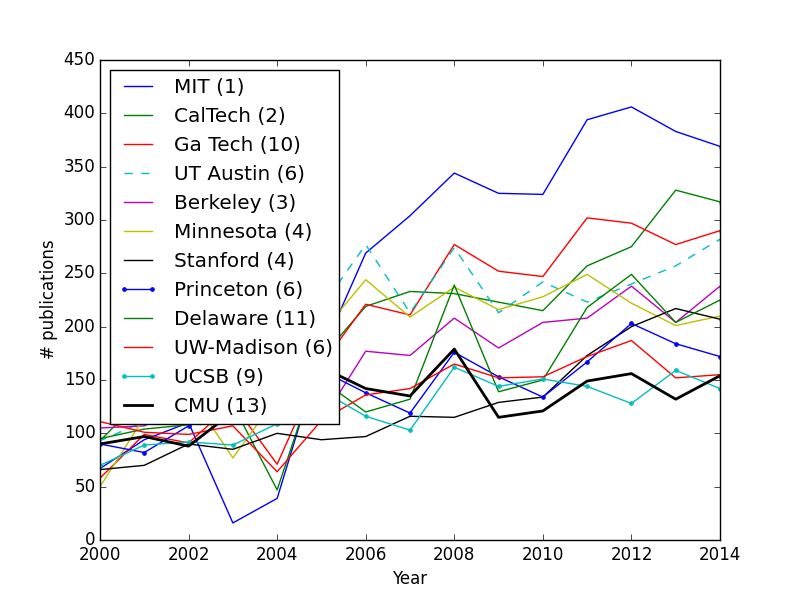
\includegraphics[width=.9\linewidth]{./redone-top-10-publications.png}
\caption{Historical number of publications for approximately the top 10 ChemE departments, including CMU. \label{fig-top10}}
\end{figure}

A comparison of the number of publications from CMU-ChemE and approximately the next 10 departments is shown in Figure \ref{fig-next10}. We are near the top of this plot, but there are a notable number of schools that publish more than us, but which are currently ranked lower.

\begin{figure}[htb]
\centering
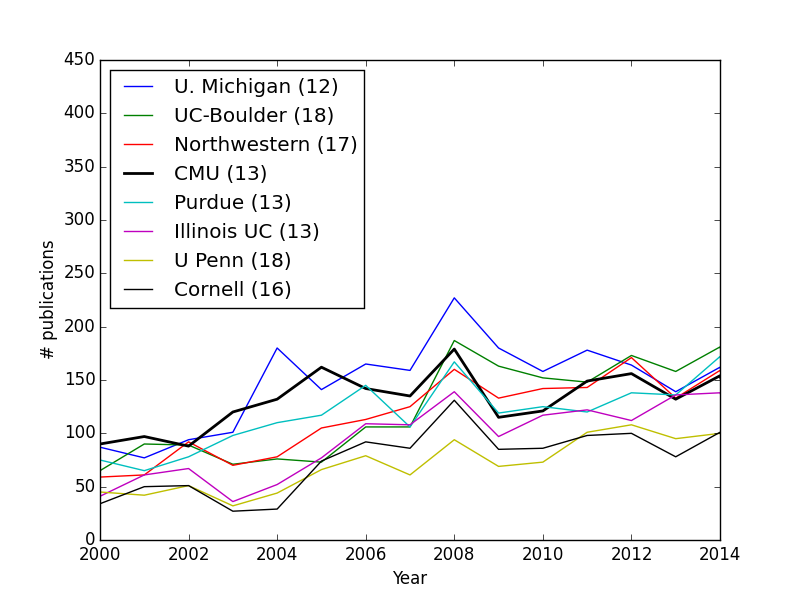
\includegraphics[width=.9\linewidth]{./redone-next-10-publications.png}
\caption{Historical number of publications for approximately the next 10 ChemE departments, including CMU. \label{fig-next10}}
\end{figure}

\subsection{MIT}
\label{sec-1-1}
\begin{center}
\begin{tabular}{lr}
Journal & \#Publications\\
\hline
ACS Nano & 12\\
Proceedings of the National Academy of Sciences of the United States of America & 11\\
ACS Applied Materials and Interfaces & 8\\
Crystal Growth and Design & 8\\
Journal of Physical Chemistry A & 8\\
Energy and Environmental Science & 7\\
Langmuir & 7\\
RSC Advances & 7\\
Advanced Materials & 6\\
Computers and Chemical Engineering & 6\\
\end{tabular}
\end{center}

\begin{center}
\begin{tabular}{lr}
count & name\\
\hline
Strano M.S. 7004189361 & 21\\
Braatz R.D. 7005734090 & 18\\
Anderson D.G. 55561679100 & 18\\
Jensen K.F. 35551829500 & 17\\
Doyle P.S. 55810114300 & 15\\
Langer R. 55763795283 & 13\\
Olsen B.D. 16310882200 & 12\\
Hammond P.T. 55197103300 & 11\\
Myerson A.S. 35586255000 & 11\\
Green W.H. 7402259989 & 11\\
\end{tabular}
\end{center}

929 citations for 2014 publications

\subsection{Caltech}
\label{sec-1-2}

\begin{center}
\begin{tabular}{lr}
Journal & \#Publications\\
\hline
Journal of the American Chemical Society & 28\\
Angewandte Chemie - International Edition & 16\\
Proceedings of the National Academy of Sciences of the United States of America & 15\\
Atmospheric Chemistry and Physics & 8\\
Chemical Science & 8\\
Polyhedron & 8\\
ACS Catalysis & 7\\
Macromolecules & 7\\
Astrophysical Journal & 6\\
Energy and Environmental Science & 6\\
\end{tabular}
\end{center}

\begin{center}
\begin{tabular}{lr}
count & name\\
\hline
Arnold F.H. 7202489032 & 20\\
Lewis N.S. 55279232600 & 17\\
Seinfeld J.H. 56133413500 & 16\\
Grubbs R.H. 36047111100 & 16\\
Stoltz B.M. 7007068441 & 15\\
Brunschwig B.S. 6701688669 & 12\\
Peters J.C. 7404191116 & 11\\
Hwang S.-J. 7404626491 & 10\\
Gray H.B. 36047602600 & 10\\
\end{tabular}
\end{center}

1094 citations for 2014 papers

\subsection{GaTech}
\label{sec-1-3}
\begin{center}
\begin{tabular}{lr}
Journal & \#Publications\\
\hline
Atmospheric Chemistry and Physics & 9\\
Applied Microbiology and Biotechnology & 8\\
Journal of Physical Chemistry C & 8\\
ACS Applied Materials and Interfaces & 7\\
Carbon & 7\\
ACS Nano & 6\\
ChemSusChem & 6\\
Advanced Functional Materials & 5\\
Journal of Membrane Science & 5\\
\end{tabular}
\end{center}

\begin{center}
\begin{tabular}{lr}
count & name\\
\hline
Koros W.J. 7102165550 & 23\\
Sholl D.S. 7006706654 & 23\\
Jones C.W. 55448095700 & 22\\
Liu L. 35262715700 & 17\\
Shin H.-D. 55545525000 & 16\\
Deng Y. 7401531091 & 14\\
Nenes A. 6701378450 & 13\\
Du G. 7201728066 & 12\\
Prausnitz M.R. 7006199362 & 11\\
Li J. 52364336200 & 9\\
\end{tabular}
\end{center}

504 citations for 2014 publications

\subsection{UT Austin}
\label{sec-1-4}
\begin{center}
\begin{tabular}{lr}
Journal & \#Publications\\
\hline
Industrial and Engineering Chemistry Research & 11\\
Polymer (United Kingdom) & 11\\
Journal of Membrane Science & 10\\
Journal of Physical Chemistry C & 9\\
Chemistry of Materials & 8\\
Journal of Materials Chemistry A & 7\\
ACS Applied Materials and Interfaces & 6\\
Journal of Physical Chemistry Letters & 6\\
Journal of the American Chemical Society & 5\\
ACS Nano & 4\\
\end{tabular}
\end{center}

\begin{center}
\begin{tabular}{lr}
count & name\\
\hline
Paul D.R. 7401665359 & 24\\
Freeman B.D. 55859868200 & 22\\
Edgar T.F. 35569277000 & 20\\
Mullins C.B. 55234573000 & 19\\
Ellison C.J. 7005195819 & 18\\
Peppas N.A. 36042831900 & 15\\
Georgiou G. 7101850711 & 11\\
Truskett T.M. 6701644278 & 11\\
Johnston K.P. 7202814438 & 10\\
Ekerdt J.G. 7005513883 & 10\\
\end{tabular}
\end{center}

752 citations for 2014

\subsection{UC Berkeley}
\label{sec-1-5}

\begin{center}
\begin{tabular}{lr}
Journal & \#Publications\\
\hline
Journal of the American Chemical Society & 17\\
Journal of Catalysis & 10\\
Journal of Physical Chemistry C & 9\\
Journal of the Electrochemical Society & 9\\
Macromolecules & 9\\
ACS Catalysis & 8\\
Energy and Environmental Science & 6\\
ChemSusChem & 5\\
Journal of Physical Chemistry B & 5\\
Metabolic Engineering & 5\\
\end{tabular}
\end{center}

\begin{center}
\begin{tabular}{lr}
count & name\\
\hline
Keasling J.D. 7005564120 & 28\\
Bell A.T. 36062590400 & 26\\
Balsara N.P. 7006013888 & 20\\
Smit B. 7102999528 & 16\\
Schaffer D.V. 7005366613 & 12\\
Iglesia E. 26643572200 & 11\\
Maboudian R. 7006616139 & 11\\
Petzold C.J. 6701791305 & 10\\
Carraro C. 22960047900 & 10\\
Adams P.D. 7403071759 & 9\\
\end{tabular}
\end{center}

727 citations in 2014 publications

\subsection{U. Minnesota}
\label{sec-1-6}
\begin{center}
\begin{tabular}{lr}
Journal & \#Publications\\
\hline
Macromolecules & 13\\
Journal of Physical Chemistry C & 8\\
Langmuir & 8\\
Physical Review B - Condensed Matter and Materials Physics & 6\\
ACS Applied Materials and Interfaces & 5\\
Industrial and Engineering Chemistry Research & 5\\
AIChE Journal & 4\\
Advanced Functional Materials & 4\\
Advanced Materials & 4\\
\end{tabular}
\end{center}

\begin{center}
\begin{tabular}{lr}
count & name\\
\hline
Bates F.S. 7103233705 & 15\\
Frisbie C.D. 7003751394 & 14\\
Tsapatsis M. 7005981012 & 13\\
Hillmyer M.A. 7004547986 & 13\\
Lodge T.P. 7103096958 & 13\\
Bhan A. 7103189488 & 12\\
Mkhoyan K.A. 6602079947 & 11\\
Leighton C. 7006523362 & 10\\
Daoutidis P. 35576381000 & 10\\
Dorfman K.D. 6701419011 & 10\\
\end{tabular}
\end{center}

416 citations in 2014 publications

\subsection{Stanford}
\label{sec-1-7}
\begin{center}
\begin{tabular}{lr}
Journal & \#Publications\\
\hline
ACS Applied Materials and Interfaces & 5\\
ACS Catalysis & 3\\
ACS Nano & 3\\
ACS Sustainable Chemistry and Engineering & 1\\
ACS Synthetic Biology & 1\\
Advanced Energy Materials & 3\\
Advanced Functional Materials & 1\\
Advanced Materials & 10\\
American Journal of Physiology - Lung Cellular and Molecular Physiology & 1\\
Analytical Chemistry & 2\\
\end{tabular}
\end{center}

\begin{center}
\begin{tabular}{lr}
Name & count\\
\hline
Bao Z. 55628573453 & 27\\
Norskov J.K. 7007042214 & 20\\
Jaramillo T.F. 6603398169 & 16\\
Bent S.F. 7006463092 & 15\\
Cui Y. 35207974600 & 15\\
Abild-Pedersen F. 55991126900 & 13\\
Bao Z. 23065783000 & 12\\
Kim W.-H. 55786438800 & 11\\
Frank C.W. 7201796097 & 11\\
Zheng G. 50761578600 & 11\\
\end{tabular}
\end{center}

899 citations for 2014 publications

Notes: Bao Z. has multiple Scopus IDs, so is listed twice here.

\subsection{U Delaware}
\label{sec-1-8}
\begin{center}
\begin{tabular}{lr}
Journal & \#Publications\\
\hline
ACS Catalysis & 6\\
ACS Macro Letters & 6\\
ACS Sustainable Chemistry and Engineering & 1\\
ACS Synthetic Biology & 1\\
AIChE Journal & 2\\
Advanced Functional Materials & 1\\
Advanced Materials & 1\\
Analytical Chemistry & 1\\
Angewandte Chemie - International Edition & 2\\
Annual Review of Chemical and Biomolecular Engineering & 1\\
\end{tabular}
\end{center}

\begin{center}
\begin{tabular}{lr}
count & name\\
\hline
Vlachos D.G. 7101636618 & 25\\
Wagner N.J. 7103202899 & 17\\
Yan Y. 7404585698 & 17\\
Chen J.G. 7501891385 & 16\\
Porcar L. 7004382097 & 12\\
Lobo R.F. 7201418960 & 11\\
Nikolakis V. 6602728656 & 10\\
Furst E.M. 7003449776 & 10\\
Brown C.M. 7408312784 & 10\\
Sandler S.I. 7201423885 & 9\\
\end{tabular}
\end{center}

549 citations on 2014 publications

\subsection{UC Boulder}
\label{sec-1-9}
\begin{center}
\begin{tabular}{lr}
Journal & \#Publications\\
\hline
Journal of Pharmaceutical Sciences & 11\\
Journal of Membrane Science & 8\\
Chemistry of Materials & 7\\
Journal of the American Chemical Society & 7\\
Macromolecules & 7\\
Polymer (United Kingdom) & 6\\
Advanced Functional Materials & 5\\
Advanced Materials & 5\\
Journal of Physical Chemistry C & 5\\
Dental Materials & 4\\
\end{tabular}
\end{center}

\begin{center}
\begin{tabular}{lr}
count & name\\
\hline
Bowman C.N. 56040490700 & 25\\
Randolph T.W. 7005729819 & 16\\
Carpenter J.F. 35391333500 & 14\\
Stansbury J.W. 7006360884 & 12\\
Schwartz D.K. 7403104511 & 11\\
Anseth K.S. 56040490300 & 10\\
Gin D.L. 7006152202 & 9\\
Medlin J.W. 35608601500 & 9\\
Noble R.D. 7202389795 & 9\\
Cha J.N. 7202455766 & 9\\
\end{tabular}
\end{center}

446 citations on 2014 publications

\subsection{Princeton}
\label{sec-1-10}
\begin{center}
\begin{tabular}{lr}
Journal & \#Publications\\
\hline
Journal of Chemical Physics & 11\\
Computers and Chemical Engineering & 10\\
Chemical Communications & 5\\
Industrial and Engineering Chemistry Research & 5\\
Journal of Physical Chemistry B & 5\\
AIChE Journal & 4\\
Chemical Engineering Science & 4\\
Journal of the American Chemical Society & 4\\
Langmuir & 4\\
Physical Chemistry Chemical Physics & 4\\
\end{tabular}
\end{center}

\begin{center}
\begin{tabular}{lr}
count & name\\
\hline
Floudas C.A. 7004284720 & 30\\
Loo Y.-L. 7006896614 & 13\\
Koel B.E. 35556864000 & 11\\
Panagiotopoulos A.Z. 7006335566 & 10\\
Debenedetti P.G. 7005110339 & 10\\
Carter E.A. 7202462172 & 9\\
Register R.A. 7005741264 & 8\\
Khoury G.A. 55805414200 & 8\\
Nikoubashman A. 35389366600 & 8\\
Priestley R.D. 7003933607 & 7\\
\end{tabular}
\end{center}

340 citations on 2014 publications

\subsection{Purdue}
\label{sec-1-11}
\begin{center}
\begin{tabular}{lr}
Journal & \#Publications\\
\hline
AIChE Journal & 8\\
Journal of Catalysis & 8\\
ACS Catalysis & 6\\
Computers and Chemical Engineering & 6\\
ACS Applied Materials and Interfaces & 5\\
Industrial and Engineering Chemistry Research & 5\\
Journal of Chromatography A & 5\\
Journal of Physical Chemistry C & 5\\
Angewandte Chemie - International Edition & 4\\
Chemistry of Materials & 4\\
\end{tabular}
\end{center}

\begin{center}
\begin{tabular}{lr}
name & count\\
\hline
Agrawal R. 35236216500 & 16\\
Ribeiro F.H. 7102417820 & 14\\
Delgass W.N. 55665425600 & 11\\
Abu-Omar M.M. 7004120750 & 10\\
Miller J.T. 7501599068 & 10\\
Greeley J.P. 56268000500 & 9\\
Nagy Z.K. 7201536402 & 9\\
Ramkrishna D. 35566975200 & 9\\
Wu Y. 55552707700 & 8\\
Stach E.A. 7005363187 & 7\\
\end{tabular}
\end{center}

267 citations on 2014 publications

\subsection{U Michigan}
\label{sec-1-12}
\begin{center}
\begin{tabular}{lr}
Journal & \#Publications\\
\hline
PLoS ONE & 6\\
ACS Nano & 5\\
ACS Applied Materials and Interfaces & 4\\
Industrial and Engineering Chemistry Research & 4\\
Journal of Power Sources & 4\\
Journal of Rheology & 4\\
Nano Letters & 4\\
Soft Matter & 4\\
ACS Sustainable Chemistry and Engineering & 3\\
Advanced Materials & 3\\
Applied Catalysis B: Environmental & 3\\
Catalysis Today & 3\\
Energy and Fuels & 3\\
\end{tabular}
\end{center}

\begin{center}
\begin{tabular}{lr}
count & name\\
\hline
Savage P.E. 7202875052 & 17\\
Larson R.G. 7402161971 & 15\\
Kotov N.A. 22135180200 & 12\\
Monroe C.W. 7006243205 & 11\\
Glotzer S.C. 7004361447 & 11\\
Lahann J. 6603555265 & 9\\
Engel M. 7102289204 & 6\\
Schwank J.W. 7006239108 & 6\\
Cheng C. 55505228000 & 6\\
Zhao C. 7403563969 & 6\\
\end{tabular}
\end{center}

313 publications on 2014 publications

\subsection{Northwestern}
\label{sec-1-13}
\begin{center}
\begin{tabular}{lr}
Journal & \#Publications\\
\hline
Industrial and Engineering Chemistry Research & 8\\
AIChE Journal & 7\\
Chemical Communications & 6\\
Biomaterials & 5\\
Computers and Chemical Engineering & 5\\
ACS Synthetic Biology & 4\\
Biotechnology and Bioengineering & 4\\
Journal of Physical Chemistry C & 4\\
Journal of the American Chemical Society & 4\\
Catalysis Letters & 3\\
\end{tabular}
\end{center}

\begin{center}
\begin{tabular}{lr}
count & name\\
\hline
You F. 24451544800 & 20\\
Shea L.D. 7005328686 & 19\\
Snurr R.Q. 7004265176 & 18\\
Broadbelt L.J. 7005682410 & 13\\
Kung H.H. 7402514104 & 12\\
Kung M.C. 7102775676 & 9\\
Jewett M.C. 7004518193 & 8\\
Yue D. 55376757800 & 7\\
Hupp J.T. 7101807715 & 6\\
Shen J. 55488336900 & 6\\
\end{tabular}
\end{center}

392 citations on publications

\subsection{CMU}
\label{sec-1-14}
\begin{center}
\begin{tabular}{lr}
Journal & \#Publications\\
\hline
Computers and Chemical Engineering & 27\\
Industrial and Engineering Chemistry Research & 16\\
AIChE Journal & 12\\
Atmospheric Chemistry and Physics & 5\\
Journal of Applied Physics & 4\\
Surface Science & 4\\
Applied Energy & 3\\
Environmental Science and Technology & 3\\
Journal of Physical Chemistry C & 3\\
Atmospheric Environment & 2\\
Atmospheric Measurement Techniques & 2\\
Carbon & 2\\
\end{tabular}
\end{center}

\begin{center}
\begin{tabular}{lr}
Name & count\\
\hline
Grossmann I.E. 7102750465 & 42\\
Biegler L.T. 7006104981 & 20\\
Pandis S.N. 7006023094 & 11\\
Jhon M.S. 7005439331 & 8\\
Sahinidis N.V. 7004139208 & 7\\
Gellman A.J. 35514271900 & 7\\
Kitchin J.R. 7004212771 & 7\\
Ydstie B.E. 7006234601 & 7\\
Martin M. 35307425700 & 6\\
Wassick J.M. 7801493949 & 5\\
\end{tabular}
\end{center}

198 citations for 2014 publications

\subsection{Illinois}
\label{sec-1-15}
\begin{center}
\begin{tabular}{lr}
Journal & \#Publications\\
\hline
PLoS ONE & 7\\
Langmuir & 5\\
ACS Catalysis & 4\\
Angewandte Chemie - International Edition & 3\\
Applied and Environmental Microbiology & 3\\
Biotechnology and Bioengineering & 3\\
Journal of Chemical Physics & 3\\
Journal of the American Chemical Society & 3\\
Metabolic Engineering & 3\\
Molecular Microbiology & 3\\
\end{tabular}
\end{center}

\begin{center}
\begin{tabular}{lr}
Name & count\\
\hline
Zhao H. 7404778848 & 25\\
Kenis P.J.A. 6701733846 & 14\\
Kong H. 7201353008 & 9\\
Rao C.V. 55362704500 & 7\\
Yang H. 35783639600 & 6\\
Harley B.A.C. 7003442002 & 6\\
Desai A.V. 36645766500 & 5\\
Seebauer E.G. 7004424518 & 5\\
Pack D.W. 7005113394 & 5\\
Lian J. 24553907300 & 4\\
\end{tabular}
\end{center}

258 citations for 2014 publications

\subsection{UCSB}
\label{sec-1-16}
\begin{center}
\begin{tabular}{lr}
Journal & \#Publications\\
\hline
Macromolecules & 7\\
Diabetes Technology and Therapeutics & 6\\
Journal of Chemical Physics & 6\\
ACS Nano & 5\\
Journal of Controlled Release & 5\\
Langmuir & 5\\
Soft Matter & 5\\
ACS Macro Letters & 4\\
AIChE Journal & 4\\
Chemistry of Materials & 4\\
\end{tabular}
\end{center}

\begin{center}
\begin{tabular}{lr}
count & name\\
\hline
Dassau E. 8613444900 & 14\\
Mitragotri S. 7004334682 & 13\\
Kramer E.J. 55588362100 & 12\\
Doyle III F.J. 35232822700 & 10\\
Doyle F.J. 35232822700 & 10\\
Israelachvili J.N. 23035044700 & 10\\
Fredrickson G.H. 7005460604 & 9\\
Squires T.M. 7005606427 & 8\\
Leal L.G. 7103037972 & 8\\
Jovanovic L. 34770955700 & 7\\
\end{tabular}
\end{center}

267 citations for 2014 publications

\subsection{UPenn}
\label{sec-1-17}
\begin{center}
\begin{tabular}{lr}
Journal & \#Publications\\
\hline
Langmuir & 9\\
Proceedings of the National Academy of Sciences of the United States of America & 5\\
Industrial and Engineering Chemistry Research & 4\\
Soft Matter & 4\\
ACS Applied Materials and Interfaces & 3\\
Blood & 3\\
Integrative Biology (United Kingdom) & 3\\
ACS Nano & 2\\
Applied Catalysis A: General & 2\\
Biophysical Journal & 2\\
\end{tabular}
\end{center}

\begin{center}
\begin{tabular}{lr}
count & name\\
\hline
Lee D. 8882507400 & 17\\
Gorte R.J. 7005801370 & 15\\
Diamond S.L. 7202852214 & 10\\
Hammer D.A. 55537179900 & 7\\
Riggleman R.A. 14054798300 & 7\\
Lazzara M.J. 6602073517 & 5\\
Cargnello M. 35335926300 & 5\\
Vohs J.M. 56262596400 & 4\\
Radhakrishnan R. 7103113008 & 4\\
Stebe K.J. 7004561002 & 4\\
\end{tabular}
\end{center}

166 citations on 2014 publications
% Emacs 24.4.1 (Org mode 8.2.10)
\end{document}